\chapter{Literature review}

This chapter should give the reader an overview of the components required for global illumination.
One will give an introduction to all required topics for path tracing. Nonetheless, for the sake of the scope, it is not as detailed as technical literature. 
Hence, if concepts or terms are unclear, one has to revise those accordingly.

\section{Rendering}

\begin{figure}[h]
\centering
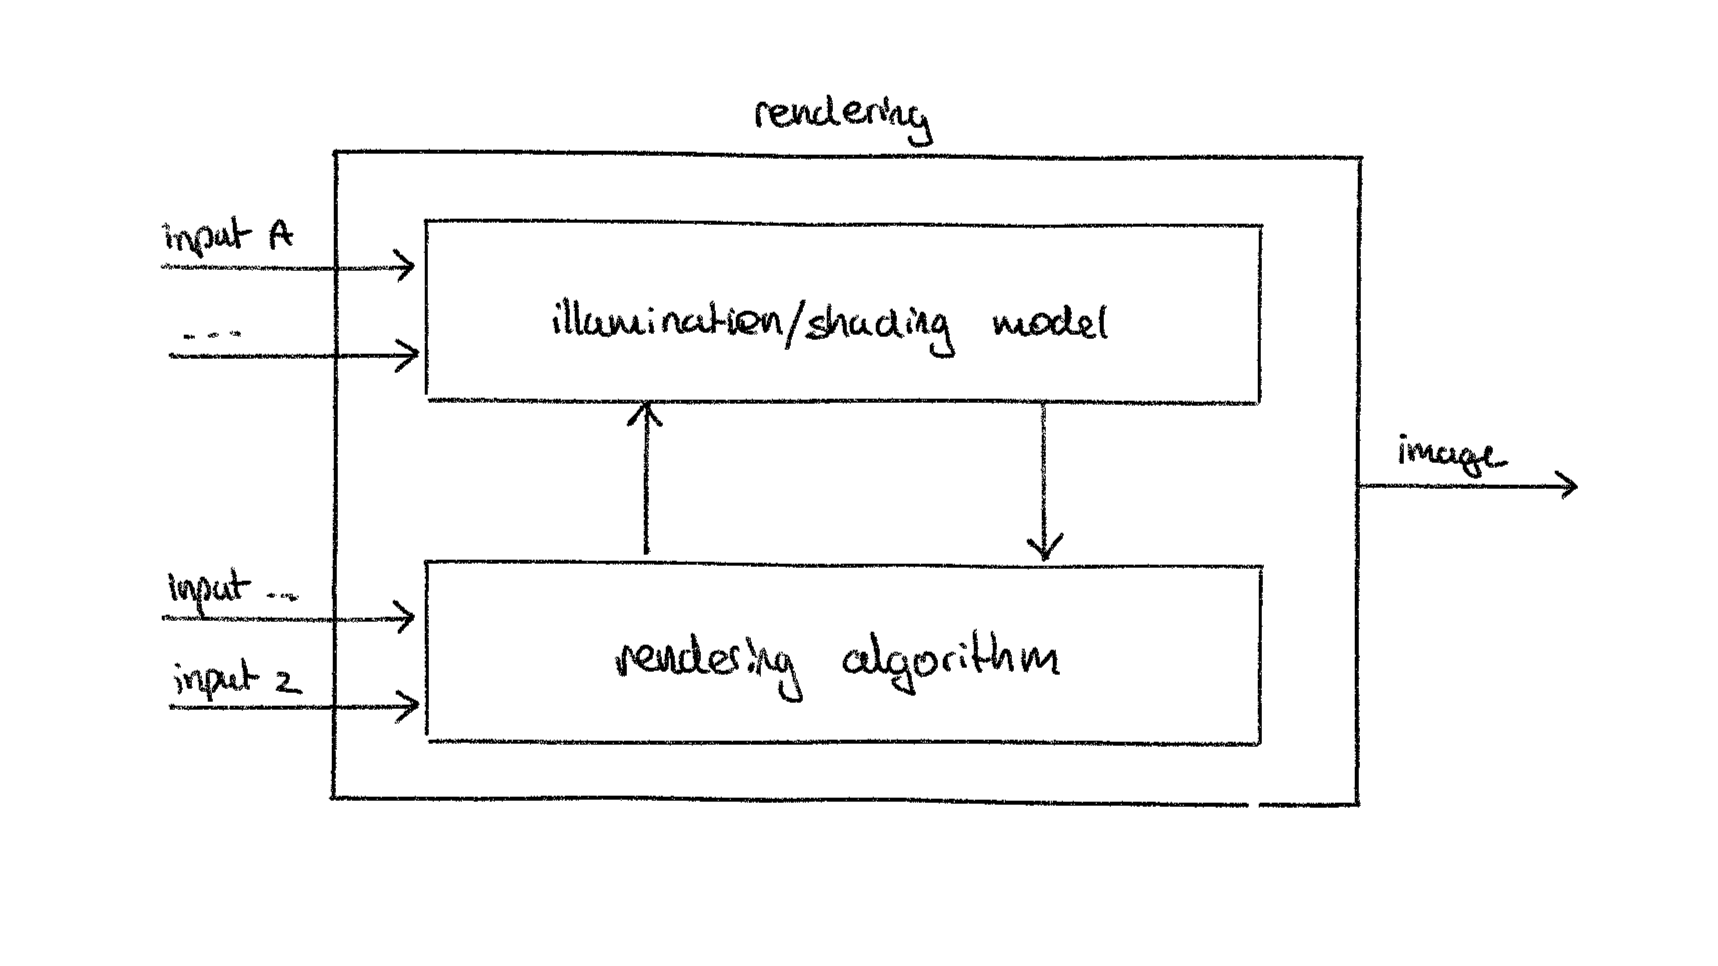
\includegraphics[width=0.9\textwidth]{rendering.png}
\caption[]{rendering composition \cite{duin_beleuchtungsalgorithmen_1993}}
\label{fig:rendering}
\end{figure}

Rendering is the process of synthesising images. 
It consists of an illumination model and a rendering algorithm.
Together they enable one to synthesise images with different properties depending on the selected model or algorithm.
Thus, one has to be careful when selecting these components because, depending on the use case, less or more sophisticated components are desirable.

For this thesis, one wants to create realistic images regarding surface responses.
A possible procedure is path tracing (section \ref{sec:path-tracing}) in combination with the Disney illumination model (section \ref{sec:disney-illumination-model}).
The following sections will elaborate on these components.

\section{Monte Carlo Integration}

In the book, \textit{Physically Based Rendering} \cite{pharr_physically_2017}, the authors explained that the integral, as a complex mathematical operator, opposes a challenge in computer science leading to numerous issues. 
Furthermore, they described that traditional methods like trapezoidal integration and the midpoint method are sufficient for low-dimensional and differentiable functions; however, these methods show a poor convergence rate for functions not fulfilling the criteria.
Nonetheless, approximations with numerical methods are the only solution to evaluate such terms due to the finite resources computers have.

Path Tracing uses the Monte-Carlo integration because it has many practical properties presented later.
As with all Monte-Carlo techniques, illustrated by \cite{kalos_monte_2008}, it does use randomness for repeated random sampling to find an accurate solution on average.

Therefore, one gives a quick overview of probability theory to understand how the integration method works.

\subsection*{Probability Theory}

A \textbf{random variable} is a function that maps a random process to a real-valued number, and one denotes it with a capitalised letter.
The \textbf{cumulative distribution function} $F(x)$ gives the probability for a random variable $X$ that is less than or equal to a value $x$.

\begin{align*}
F(X)=Pr\{X\le x\}
\end{align*}

Using calculus, one can differentiate $F(x)$, if possible, yielding the \textbf{probability density function} $f(x)$.
The density function describes the likelihood for a random variable to be in an interval $[a,b]$.

\begin{align*}
f(x)=\frac{dF(x)}{dx}
\end{align*}

The \textbf{expected value} is a weighted average, which is evaluable for a random variable.
This requires the cumulative distribution $F(x)$ and corresponding density function $f(x)$.

\begin{align*}
E[X]=\int_{\Omega}F(x)\,f(x)\,dx
\end{align*}

The final metric is the \textbf{variance} which gives the mean squared deviation.

\begin{align*}
V[X]=E\left[(x-E[x])^2\right]
\end{align*}

\subsection*{Monte-Carlo Estimator}

Given is:

\begin{align*}
F=\int f(x)\,dx\quad\text{where}\quad f:D \mapsto R
\end{align*}

The task is to find an answer for the integral where $f(x)$ is a function that can take on any form.
The concept, as explained before, is to have a random variable $X:\Omega\mapsto\mathbb{R}$ where $\Omega$ is a set of all possible outcomes mappable to a real-valued number.
Additionally, one assumes that samples are uniformly distributed over an interval $[a,b]$.
Now, one uses the random variable $X$ as an input for the function $f$ and accumulates the results of $f$.
Based on that, one can derive the following estimator:

\begin{align*}
F_N=\frac{b-a}{N}\sum_{i=1}^{N}f(X_i)
\end{align*}

Currently, the estimator allows only for uniformly sampled values in an interval.
However, to generalise it, select a random variable with a probability density $p(x)$ that can weight $f(x)$.

\begin{align}
F_N=\frac{1}{N}\sum_{i=1}^{N}\frac{f(X_i)}{p(X_i)} \label{eq:mc-estimator}
\end{align}

Elaborating on eq.~\ref{eq:mc-estimator}, one can identify $F_N$ as a random variable which depends on the size of $N$, and $N$ sets the number of samples.
Note that $F_N \approx F$ and $F_N$ will be accurate on average.
One can show the accuracy with the expected value.

\begin{align*} 
E[F_N] &=E\left[\frac{1}{N}\sum_{i=1}^{N}\frac{f(X_i)}{p(X_i)}\right]\\
&=\frac{1}{N}\sum_{i=1}^{N}E\left[\frac{f(X_i)}{p(X_i)}\right]\\
&=\frac{1}{N}\sum_{i=1}^{N}\int_{a}^{b}\frac{f(x)}{p(x)}\,p(x)\,dx\\ &=\int_{a}^{b}f(x)\,dx 
\end{align*}

Now, one gives a quick overview of the advantages and disadvantages and quickly explains why these are useful.

Veach \cite{veach_robust_1997} pointed out the essential advantages and disadvantages of the Monte-Carlo integration.
The first point mentioned was the convergence rate of the estimator.
He showed that the estimator converges with the rate of $O(N^{-1/2})$ for high dimensional integrals with discontinuities.
This vital attribute even applies to an estimator with infinite variance. 
In other words, convergence is slow but guaranteed.
Nonetheless, based on that, one can determine the required samples to reduce the error by half.
Accordingly, one can conclude that it needs four times more samples to decrease the error while increasing runtime substantially.
However, Veach presented optimisations which allow for a more efficient convergence, see the upcoming section.
The second benefit is the simplicity of the algorithm.
He explained that this qualifies for flexible design with an integrator that is a black box.
This fact is essential as one can separate procedure from technical details.
The result is that the algorithm's implementation happens once, and the meaning of the data is unrelated, making it suitable for various problems requiring integration.
The last two traits are that Monte-Carlo can theoretically handle any domain, even an infinite-dimensional space, and work with integrands with singularities.

\subsection*{Optimisation}

The final part of the Monte-Carlo integration is about optimisations, as these play a considerable part in making this technique feasible for multiple applications.

The drawback of this technique is random sampling because the result depends on the number of drawn samples.
Consequently, a large sample count will produce more accurate results with a minor variance but increasing runtime.
The goal is to increase the efficiency of an estimator by reducing variance or runtime.

Before exploring techniques for variance reduction, one must clarify what efficiency means.

\begin{align}
\epsilon[F]=\frac{1}{V[F]\,T[F]}
\label{eq:estimator-eff}
\end{align}

Veach explained that one tries to find an estimator where variance and runtime are neglectable, and the eq.~\ref{eq:estimator-eff} describes this as a trade-off with $V[F]$ being the variance and $T[F]$ time required to determine $F$; \cite{veach_robust_1997}.
Accordingly, an estimator can become more efficient if it reduces runtime or variance.

\subsubsection*{Importance Sampling}

Importance Sampling has the principle to find a probability density function $p(x)$ which is similar to the integrand $f(x)$.
Optimally, the $p(x) \propto f(x)$ and considering equation eq.~\ref{eq:mc-estimator} it would give this configuration.

\begin{align*}
\frac{f(X_i)}{p(X_i)}=\frac{f(X_i)}{c\,f(X_i)}=\frac{1}{c} \Rightarrow F_N=\frac{1}{N}\sum_{i=1}^{N}\frac{1}{c}
\end{align*}

Leftover is a constant of proportionality $c$.
The proportionality of $p(x)$ and the current configuration of the summation demands that the normalisation must be the integral's value; \cite{veach_robust_1997}.

\begin{align*}
c=\frac{1}{\int\,f(x)\,dx}
\end{align*}

Based on that, the authors of the book \cite{kalos_monte_2008} conclude that a $p(x)$ similar to $f(x)$ will lead to a tremendous variance reduction.
The decrease is due to increasing the likelihood of sampling areas where the integrand is large, contributing more to the final result.
There are some constraints for $p(x)$ where it must match the behaviour of the integrand and its upper bound with $\forall x : p(x) > f(x)$.
Caution, selecting an incorrect $p(x)$ can have the opposite effect leading to more variance.

\subsubsection*{Adaptive sample placement}

Adaptive sample placement is another option to increase the efficiency of an estimator.
The basic idea is to sample more complicated or contributing regions based on previous samples.
However, the main disadvantage pointed out by \cite{veach_robust_1997} is the introduction of bias to the estimator that could lead, as an example, to image artefacts.

A quick excurse to elaborate on the problem of bias.

\begin{align*}
\beta = E[F]-\int f(x)\,dx
\end{align*}

The bias of an estimator describes the difference between the expected value and the exact value of an integral.
For example, the original derived estimator had the property $E[F]=\int\,f(x)\,dx$ and is therefore unbias.
Modifying the equation, for example, not accounting for a particular value range, will change the expected value and automatically bias the other values.
If the bias is overly large, it causes issues like variance or even another result which is not desirable.
Nonetheless, as explained in \cite{kalos_monte_2008}, it does not matter if an estimator is biased if it helps increase its efficiency without showing a significant difference, making it feasible for more applications.

Russian roulette is a possible technique for reducing samples for regions where the integrand is low and therefore contributes less to the final result.
In \cite{pharr_physically_2017} the authors elaborated that skipping low values does not matter because the expected value is still correct on average.
Another fact they explained is that Russian roulette does not reduce variance (it can even increase it), but it improves efficiency by not evaluating less important regions; hence the runtime improves.

\section{Light Integrals}

Performing light transport simulations requires a formalisation of light.
For Path Tracing, one utilises tools from physics to create a framework.
Duin \cite{duin_beleuchtungsalgorithmen_1993} described different models of light and how each of them comes with particular strengths in modelling the light's behaviour.
He elaborated that these models, like particle dualism, are outstanding in describing the nature of light but are not necessary for computer graphics where optics and radiometry are sufficient to model light at its core.
Based on that, he stressed the idea of light propagation and explained how light traverses the scene and interacts with other objects.
A \textit{scene} is a formal description containing elements like an object, light rays and volumetrics.
An \textit{object} is a geometric model consisting of triangles representing a shell of a real object.

\subsection*{Rendering Equation}

In 1986 Kajiya \cite{kajiya_rendering_1986} proposed the famous rendering equation that describes light propagation based on physics radiative heat transfer literature.
As a general geometrical optics approximation, its purpose is to evaluate the leaving equilibrium radiance at a point $p$ in the direction $\omega_o$ from all in-coming directions $\omega_i$ with a cosine term for the projection of the solid angle and a reflectance function $f(p, \omega_o, \omega_i)$ describing attenuation of the light.

\begin{align}
L_o(x,\omega_o)=L_e(x,\omega_o)+\int_{S^2}f_r(x,\omega_o,\omega_i)\,L_i(x,\omega_i)\,\left|\cos\theta_i\right|\,d\omega_i
\label{eq:rendering}
\end{align}

See that eq.~\ref{eq:rendering} is a recursive formulation where the in-coming directions are again integrals determined at other points in the scene.
That is why there is no immediate solution to the rendering equation; however, Ray Tracing with Monte-Carlo integration, known as Path Tracing, builds the foundation to solve such a simulation problem.

\subsection*{Three-Point Form}

The rendering equation is ideal for understanding the concept of light propagation; however, unflexible to derive estimators because it is an integral over a solid angle.
Thus, let one prepare an integral over areas, the so-called three-point form; \cite{veach_robust_1997}.
Based on that, one will derive the path integral, providing more freedom in constructing an estimator.

The first step is to replace all terms in the eq.~\ref{eq:rendering} containing a direction $\omega=\widehat{x'-x}$ with $x'\rightarrow x$:

\begin{align*}
L(x,\omega)=L(x'\rightarrow x)\quad\wedge\quad f_r(x,\omega_o,\omega_i)=f_r(x''\rightarrow x'\rightarrow x)
\end{align*}

The arrow emphasises the direction of light flow; \cite{veach_robust_1997}.
The next step is to change the integral domain over an area $A$, which also changes the integration variable, including the cosine term.
In \cite{kajiya_rendering_1986}, there are self-describing figures that show the configuration of the points and directions.

\begin{align*}
d\omega=\frac{|\cos\theta'|}{\|x'-x\|^2}dA(x') \Rightarrow |\cos\theta|\,d\omega=\frac{|\cos\theta|\,|\cos\theta'|}{\|x'-x\|^2}dA(x')
\end{align*}

However, this is not yet correct because two points must be visible.
The function $V$ is a visibility function that verifies that two points are from each other visible.
One utilises the visibility function and the previous equation for a geometry term $G$. If two points are not mutually visible, then the function is 0.

\begin{align*}
G(x'\leftrightarrow x)=V(x'\leftrightarrow x)\frac{|\cos\theta|\,|\cos\theta'|}{\|x'-x\|^2}
\end{align*}

Substituting all terms in eq.~\ref{eq:rendering} gives the three-point Form.

\begin{align}
L(x'\rightarrow x)=L_e(x'\rightarrow x)+\int_{A}L(x''\rightarrow x')\,f_r(x''\rightarrow x'\rightarrow x)\,G(x''\leftrightarrow x')\,dA(x'')
\label{eq:three-point}
\end{align}

\subsection*{Path Integral}

An alternative representation of the rendering equation is the path integral.
It explains detailed rendering characteristics comprehensively, including a local sampling technique used in the implementation of this thesis.

Deriving the integral is intuitive as one can take the eq.~\ref{eq:three-point} and recursively replace the incoming radiance with the equation itself.
Rearranging the new infinite recursive equation, one can separate it into multiple elements that govern a particular function.

\begin{align}
L(x_1\rightarrow x_0)=\sum_{n=1}^\infty P(\bar{x}_n)
\label{eq:path-integral}
\end{align}

The eq.~\ref{eq:path-integral} represents the path integral.
Its task is to find the in-coming radiance at $x_0$ regarding a path $\bar{x}_n=x_0,x_1,\dotso,x_n$ with $n+1$ vertices.
Notice that it summates the total radiance of paths $P(\bar{x})$, which gives the accumulated total radiance obtained by a point $x_0$ on the camera plane.
The summation is over an infinite domain where only the subset of paths with finite length is of interest.

\begin{align}
P(\bar{x}_n)=\underbrace{\int_A \int_A \dots \int_A}_{n-1}\left(L_e(x_n\rightarrow x_{n-1})\,T(\bar{x}_n) \right)dA(x_2)\dotso dA(x_n)
\label{eq:path-radiance}
\end{align}

Eq.~\ref{eq:path-radiance} is the radiance of a paths $\bar{x}_n$.
It demands solving multiple nested integrals over areas representing all possible paths with almost any combination of vertices $x_n$ forming a valid path to a light source or the scene enclosure.

\begin{align}
T(\bar{x}_n)=\prod_{k=1}^{n-1}f(x_{k+1}\rightarrow x_k\rightarrow x_{k-1})G(x_{k+1}\leftrightarrow x_{k})
\label{eq:path-throughput}
\end{align}

Eq.~\ref{eq:path-throughput} gives the throughput $T(\bar{x}_n)$ that expresses the fraction of received radiance from a light source; \cite{pharr_physically_2017}.
This part is essential for the Monte-Carlo estimator as it explains how to keep track of the throughput state during the rendering process.

Now, one summarises the benefits before the subsequent section explains how the path integral incorporates the Monte-Carlo algorithm.

Veach \cite{veach_robust_1997} provided a detailed overview of the path integral's advantages.
The first point he described is that one can derive new rendering algorithms employing general-purpose integration techniques like importance sampling.
The second benefit is a geometric primitive, the path, which makes computation more comfortable.
Another benefit of working with paths is that they are more exact and complete regarding light transportations, as one uses the whole trajectory of light rather than distinct segments.
The construction of such paths is not limited to local information. 
That qualifies for an open selection process of path vertices.
Last, it provides a framework to work with the probability density of paths.

\section{Path Tracing} \label{sec:path-tracing}

\textit{Path tracing} is a rendering algorithm used for image synthesis.
It employs ray tracing and Monte-Carlo integration to compute paths with corresponding vertices.
At each vertex, one evaluates an illumination model.
The algorithm gives a formal definition of assembling paths for rendering.

A \textit{local sampling technique} is a definition that describes the construction of paths based on local information one at a time; \cite{veach_robust_1997}.
The easiest way is to sample directions regarding a probability density function.
One uses ray tracing to find the next vertex position.
This approach also solves the visibility problem, constructing only valid paths.
Of course, this strategy to find paths is not ideal but sufficient, making it a good choice; \cite{pharr_physically_2017}.

The only problem now is that one would sample paths using a solid angle and recollect that an angle's probability density is not the same as the probability density of an area.
Therefore, one has to make the conversion to calculate the correct probability of a path.

\begin{figure}[h]
\centering
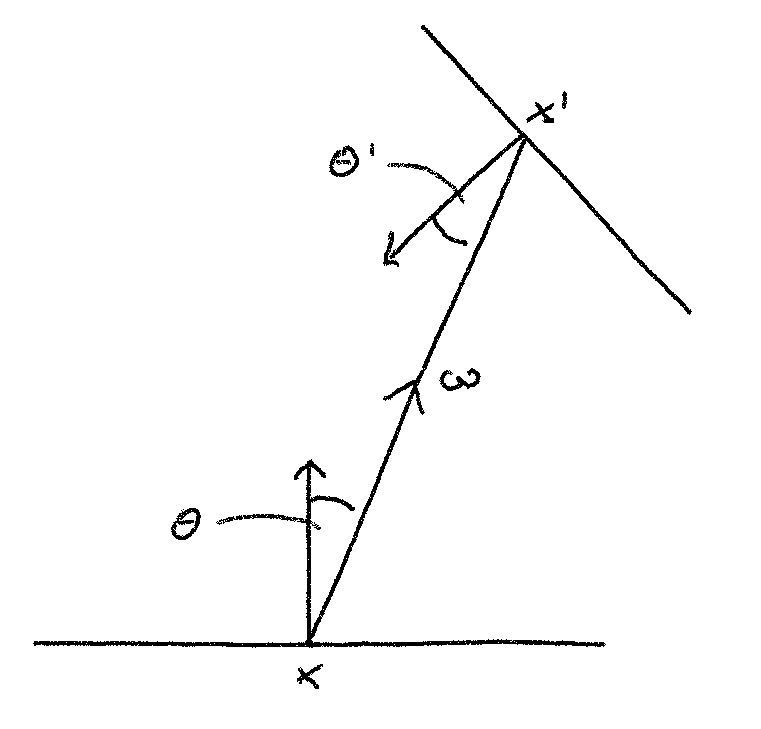
\includegraphics[width=0.33\textwidth]{sampling-configuration.png}
\caption[]{configuration of path vertices}
\label{fig:path-vertices}
\end{figure}

The figure \ref{fig:path-vertices} depicts the configuration of path vertices.
Vertex $x$ is the point of interest, and $x'$ is a potential successor.
In the present framework, one does sample a direction $\omega$ and cast a ray from $x$ towards $x'$.
Currently, one has only the probability of $\omega$. 
However, the following conversion term is applied to find the probability of $x'$.

\begin{align*}
p(x')=p(\omega)\frac{|\cos\theta'|}{\|x'-x\|^2}
\end{align*}

The authors \cite{pharr_physically_2017} illustrated how applying the conversion term to the probability density function in eq.~\ref{eq:path-radiance} causes the geometry function $G$ to cancel out partially because of the last vertex at the light source.
Remember, the last vertex originates from a distribution over the light's surface area; hence, one does not apply the conversion.

\begin{align*}
\frac{f(x_{n}\rightarrow x_{n-1}\rightarrow x_{n-2})G(x_n\leftrightarrow x_{n-1})}{p(x_n)}\,\left(\prod_{k=1}^{n-2}\frac{f(x_{k+1}\rightarrow x_{k}\rightarrow x_{k-1})|\cos\theta_{k}|}{p(\widehat{x_{k+1}-x_{k}})}\right)
\end{align*}

Using eq.~\ref{eq:path-throughput} gives the final throughput term for the present sampling framework.
Note that throughput is a combination of the reflectance function, the cosine and the probability of the incoming direction.

%\subsection*{Limitations}

%Choosing a local sampling technique does constrain paths to the local information one provides.
%Accordingly, only a subset of valid visible paths contributes to the final image, resulting in the issue that one cannot appropriately represent all light effects.
%Veach \cite{veach_robust_1997} discussed the limitations of rendering algorithms, even demonstrating distinct scenarios where the sampling is flawed.

\section{Disney Illumination Model} \label{sec:disney-illumination-model}

Now, one will cover the Disney bidirectional distribution function (BSDF) resembling the illumination model.
Before elaborating on this model, one will give a general overview of relevant topics.

\subsection*{Illumination Models}

In computer graphics, illumination models, sometimes called shading models, provide a specification to find the directional dependent radiance of a point; \cite{duin_beleuchtungsalgorithmen_1993}, or in other words, determine how a surface responds to light.

For global illumination, one already selected path tracing as the rendering algorithm.
Now, one has to pick a shading model that accurately represents surface properties with correct responses.
Only then it is possible to re-create global illumination effects.

In the past decades, research developed many models that can successfully represent different types of surfaces.
The Disney shading model is one of these.

\subsection*{Conservation of Energy}

The conservation of energy states that a quantity, here energy of light, must stay constant in a closed system, which is, in this case, a ray-traced scene.

Note that light is a quantum object; hence the energy of such object is described by $E = h \cdot f$ where $E$ is energy, $h$ the Plank constant and $f$ is the frequency.
Due to that, one has to handle conversions of energy appropriate; otherwise, a synthesised image will be inaccurate.

Accordingly, if a light quantum hits an object, a part converts to heat, and another part energises atoms of the surface.
The light quantum keeps the amount of energy left after these conversions.
Therefore, considering light models that are energy conserving helps to create realistic coherent images without ad hoc solutions.

\subsection*{Microfacet Theory}

Trowbridge and Reitz \cite{trowbridge_average_1975} presented a model for the ray tracing theory describing rough surfaces.
It assumes that surfaces consist of microscopic details where the structure and alignment determine the appearance, hence the surface's response.
One describes the microscopic details with so-called facets.
These facets are flat shapes that only reflect light.
Thus, only a portion of the incoming light reflects on rough surfaces because all these facets have arbitrary orientations.
Research further refined the model because it produced \textit{realistic} results and accurately represented surface-light interactions.

\begin{figure}[h]
\centering
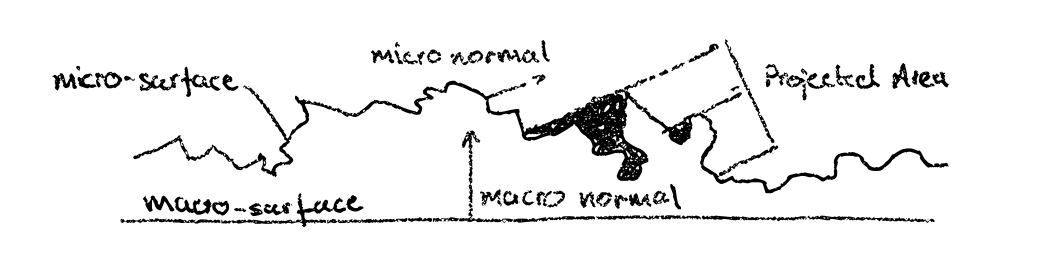
\includegraphics[width=0.6\textwidth]{microfacet-model.png}
\caption[]{Microfacet Model \cite{heitz_understanding_2014}}
\label{fig:microfacet-normal}
\end{figure}

The fig.~\ref{fig:microfacet-normal} depicts the configuration of the microfacets and the actual geometry.
As one can observe, one utilises a function $D(\omega_m)$ that describes the microscopic details (microfacets) dependent on the geometric normal $\omega_m$.
$D$ is a normal distribution function giving the probability of a facet having a particular direction.
However, this is not enough to fully describe the microfacet surface.
One has to account for self-shadowing and non-visible facets due to orientation.
Hence, a shadowing-masking function $G$ models this behaviour.
The last part of the figure is the distribution of visible microfacets $D_{\omega_o}$.
It is a projection of the microfacet surface regrading the direction $\omega_o$.

\subsection*{Philosophy}

Burley \cite{burley_physically_2012} gave a detailed overview of the goals of the new illumination model.
He created a set of guidelines that shaped the decision-making process to restrict the selection of light models (analytical and empirical) for a new illumination model.
The most notable fact is that the model is not required to be physically accurate in favour of art directable materials.
A final product is an illumination model that follows physics principles and should be physically plausible whilst fulfilling the need for artistic controls.

Accordingly, Burley presented five principles for the Disney BRDF \cite{burley_physically_2012}.
The model should be intuitive and have a minimal amount of parameters where each parameter ranges between zero and one.
The parameters can go beyond the range, and a combination of all is robust and plausible to a certain extent.

In the original paper, Burley \cite{burley_physically_2012} settled down with ten parameters to control the appearance.
However, one assumes that this changed with the latest paper that introduced transmission and subsurface scattering; \cite{burley_extending_2015}. 

\subsection*{Light Responses}

Burley used the MERL BRDF database which contains captured data of materials for different light-camera configurations to observe and evaluate physic models; \cite{matusik_data-driven_2003}, \cite{burley_physically_2012}.
Burley gave an in-depth view of the gathered observations to illustrate the decision-making process.
One will summarise the different lobes and components Disney uses for their material.

\begin{figure}[h]
\centering
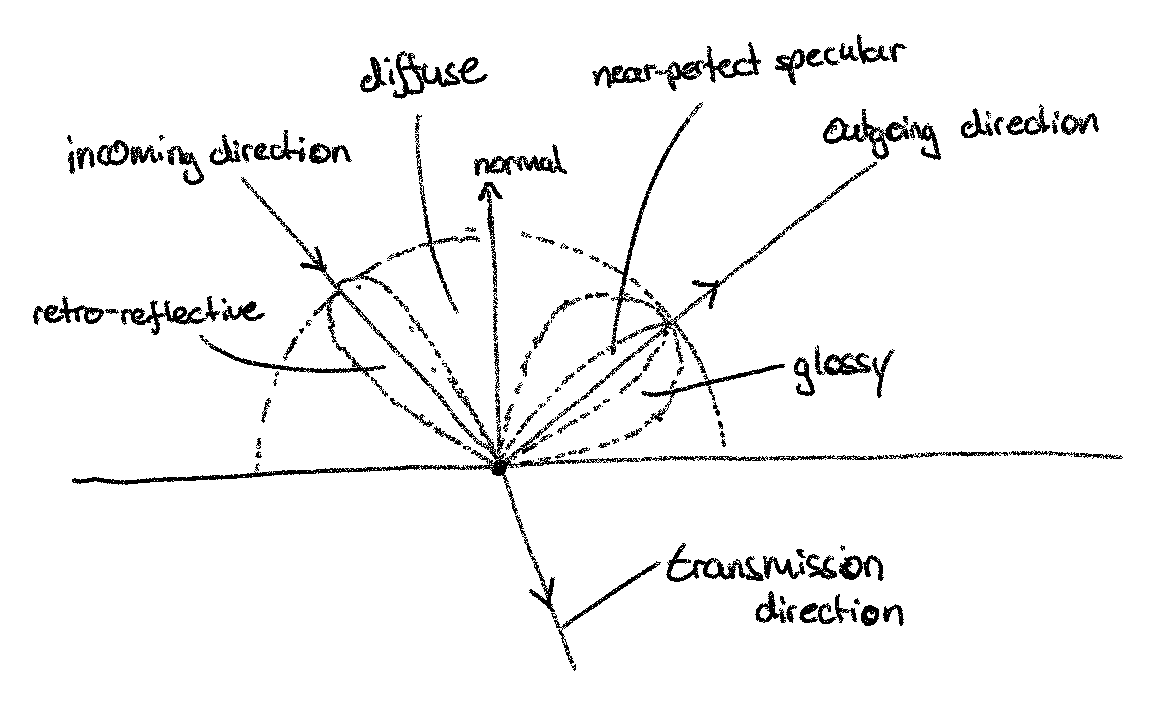
\includegraphics[width=0.75\textwidth]{bsdf-lobes.png}
\caption[]{light lobes}
\label{fig:lobes}
\end{figure}

One will follow the idea that light is categorisable into so-called light lobes.
This abstraction allows for the selection of different models governing a specific lobe's behaviour.
Regardless, natural materials often combine all categories; \cite{cook_reflectance_1982}.
Nevertheless, the abstraction enables one to handle the complexity.
There are five categories present in the Disney model: diffuse, retro-reflective, specular and transmissive.

\subsubsection*{Diffuse and Retro-Reflection}

The diffuse surface response generally represents any light that hits a non-metallic surface, which is then absorbed and re-emitted.
The absorption of specific wavelengths has two effects.
A surface reflects other wavelengths and can re-emit light due to the energised atoms.
Burley did a comparison \cite{burley_physically_2012} of the Lambert reflectance \cite{lambert_lamberts_1892} and the measured data.
He explained that Lambert diffuse loses light's directionality, which yields a constant value.
Because of that, one cannot correctly represent the surface response at the grazing angle, which needs to become darker or brighter depending on the retro-reflectiveness, which correlates to the surface roughness.
Thus, he suggested utilising a Fresnel term to re-create the response with the Lambert diffuse and a retro-reflection term.
To clarify what retro-reflection means it describes reflected light along the incident direction; \cite{berns_event_2021}.

Based on that, Burley \cite{burley_extending_2015} created two lobes, a diffuse lobe with Lambert reflectance and a retro-reflection lobe with a self-developed empirical model, where both utilise a Fresnel weight.
Besides that, he accounted for subsurface scattering so that the subsurface scattering converges against the diffuse lobe for small scattering distances.
Additionally, both lobes preserve microfacet effects needed for the specular lobe. 

\subsubsection*{Specular}

The specular lobe utilises the microfacet theory and the observations as decisions correlate to the components of the theory.

Burley \cite{burley_physically_2012} began with the distribution function $D$ and compared multiple traditional models with the measured data.
He noticed that all models had an issue replicating the peak, especially the highlights' tail (Beckmann, Blinn Phong).
That is why Walter introduced the popular GGX model, specifically creating broad tails; \cite{walter_microfacet_2007}.
Nonetheless, it is not wide enough for most materials.

Due to the difficulties, Burley adapted a Generalised-Trowbridge-Reitz (GTR), where an exponent controls the width of the distribution.
Besides that, the model offered a normalised distribution with a closed-form integral and support for importance sampling.
A revision in 2014 (B.2 GTR eq. 10) \cite{burley_physically_2012} changed the equation to account for anisotropic material behaviour.

The second term for the microfacets is the Fresnel factor which controls the specular reflection dependent on the angle difference between view and light vector as surface roughness.
Burley observed that every measured material had specular reflection at a $\theta_d=90$ where some increased significantly.

Therefore, Burley \cite{burley_physically_2012} introduced the Fresnel term utilising the Schlick approximation \cite{schlick_inexpensive_1994}.
It was sufficient owing to minor errors whilst replacing the overcomplicated entire Fresnel equation.
The introduction of a transmissive specular lobe \cite{burley_extending_2015} required the use of the entire Fresnel equation because the approximation error led to non-plausible refractions for a low index of refraction.
However, this change only applies to the primary specular lobes whilst utilising the Schlick approximation for the other lobes.

Lastly, one has to consider the geometry term $G$ that governs the light direction's shadowing and the viewing direction's masking.
Burley explained \cite{burley_physically_2012} that one cannot directly evaluate the $G$ term because it demands accurate $D$ and $F$ terms as well as a clear separation of the diffuse and specular lobe.
However, he used the directional albedo of the surface to identify the influence of the $G$ term.
The result is that most materials have a small albedo value and remain constant as a flat line up to 70 degrees regarding the incoming light's direction.
Afterwards, depending on the roughness, most materials increased or decreased in directional albedo.
He stressed that the $G$ factor has a "profound" effect on the albedo and, consequentially, the surface appearance.

Burley used an analytical model using the approach by Smith. 
It lets one derive the geometry term $G$ from the microfacet distribution $D$ if one facilitates the assumptions about geometric shadowing.
A solution by Heitz \cite{heitz_understanding_2014} replaced the used version by Burley because he accounted for anisotropy and removed the alpha-roughness conversion; (Addenda) \cite{burley_physically_2012}.

\subsubsection*{Other}

Besides the three major lobes, Disney included two minor to support visual fidelity.
Both introduced in \cite{burley_physically_2012} remained unchanged; \cite{burley_extending_2015}.

Burley supplemented the primary specular lobe with a secondary lobe to create a clearcoat layer for non-metallic materials adding extra reflections.
It increases energy by a minimal amount, but this is not a problem as it has a substantial visual impact.

One added a sheen lobe for extra grazing reflections to compensate for potentially missing specular or diffuse responses.
Accordingly, it has a Fresnel-like shape only effect grazing angles.
It is possible to tint the sheen towards the base colour.
